\documentclass[tikz,border=8pt]{standalone}
\usetikzlibrary{arrows.meta,positioning,shapes.geometric,calc}
\begin{document}
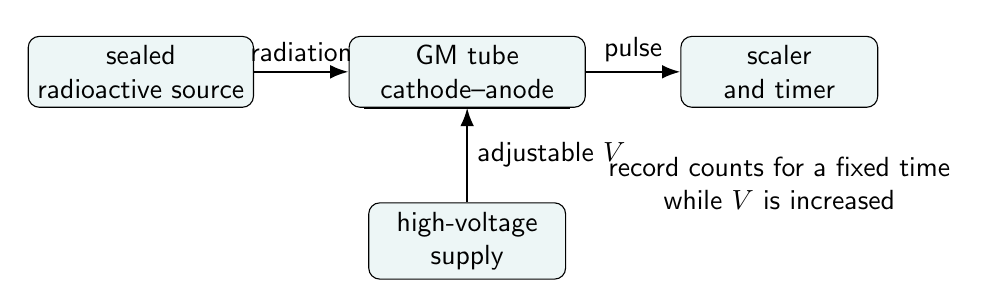
\begin{tikzpicture}[font=\sffamily,>=Latex,box/.style={draw,rounded corners,minimum height=9mm,minimum width=25mm,align=center,fill=teal!7},wire/.style={->,thick}]
\node[box] (source) {sealed\\radioactive source};
\node[box,right=12mm of source,minimum width=30mm] (tube) {GM tube\\cathode--anode};
\node[box,right=12mm of tube] (scaler) {scaler\\and timer};
\node[box,below=12mm of tube] (hv) {high-voltage\\supply};
\draw[wire] (source)--node[above]{radiation}(tube);
\draw[wire] (tube)--node[above]{pulse}(scaler);
\draw[wire] (hv)--node[right]{adjustable $V$}(tube);
\draw[thick] ($(tube.south west)+(2mm,0)$)--($(tube.south east)+(-2mm,0)$);
\node[below=5mm of scaler,align=center] {record counts for a fixed time\\while $V$ is increased};
\end{tikzpicture}
\end{document}
